	
\subsection{Current state of own research and professional competences for the project}
\label{sec:own-research}
% 1000 words

\begin{figure}[h]
	\centering
	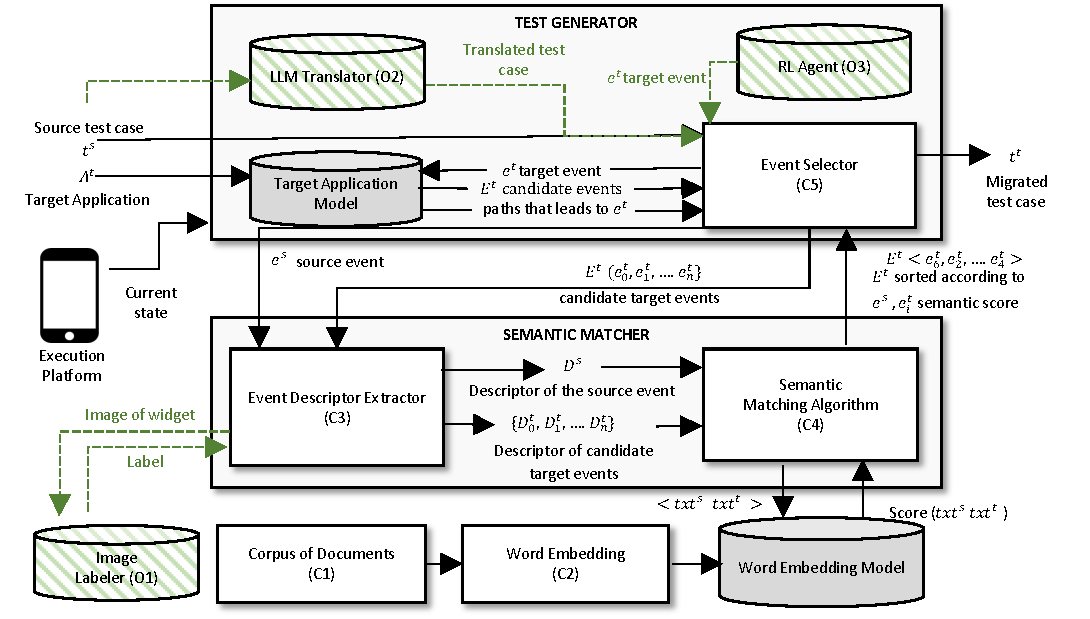
\includegraphics[width=\textwidth]{images/architecture.pdf}
	\caption{\testreuse architecture and project objectives}
	\label{fig:architecture}
\end{figure}

%Test Reuse architecture
We reviewed state-of-the-art \testreuse approaches for Android, \atm~\cite{behrang:apptestmigrator:ASE:2019}, \craftdroid~\cite{lin:craftdroid:ASE:2019}, and \adaptdroid~\cite{Mariani:Adaptdroid:AST:2021} by full replication of their experiments, and careful inspection of their source code that is publicly available.
We proposed a general \architecture for \testreuse based on our review that abstracts common components of \testreuse approaches and their interactions. 
The \architecture enables us to study \testreuse approaches in more depth, and guide researchers in developing new approaches.
C1, C2, C3, C4, and C5 are the components that we identified in the current approaches and O1, O2, and O3 (in hashed green) are the realization of \project objectives that we explain in section \ref{sec:detailed-plan}. 


% Test Ruse work flow
\bigskip
\testreuse  includes two coarse grain parts: \generator and \matcher, which collaborate to migrate source test case $t^s$ to target test case $t^t$.
\generator receives the $t^s$ and selects a match for each source event $e^s \in t^s$ in the target application $A^t$.
For each $e^s$, the \generator considers a set of target candidate event $E^t$ from the \tam and the current GUI state. 
Then, it queries the \matcher to sort the candidates based on their similarity to the $e^s$.
\generator selects an event from the sorted candidates and executes the event, transforming the current GUI state to another. 
After iterating over all the $e^s \in t^s$, the selected target events from $A^t$ comprise the migrated test case.



\bigskip
In more detail, the \generator statically analyzes $A^t$ to create a \tam and updates the model as it progresses in migrating $t^s$.
The \selector gathers a set of target candidate events $E^t$ for each event $e^s$ and selects from the candidates, which are sorted by \matcher.
If the \selector selects an event from the current GUI state, it executes the event and adds the event to the migrated test case.
If the \selector selects an event from the \tam, the event is absent in the current state and the \selector queries the \tam to find a path to the state where the selected event exists.
Then, it executes the selected events (including the stepping events) and adds them to the set of migrate test cases.
If the \selector does not select any event from $E^t$, it will skip the $e^s$.
\testreuse approaches implement the \selector strategy differently.


\bigskip
The \matcher receives a query containing the $e^s$ and $E^t$, then the \ede (C3) extracts descriptors of events $D$.
A descriptor consists of textual attributes associated with the widget of an event such as \textit{resource-id}.
For each pair of $\langle D^s,  ~D_i^t\rangle$, the \sma queries the \wem to score similarity of their textual attribute, then it aggregates the scores to sort the $E^t$.
The \wem encodes words (or sentences) to vectors, representing the semantic distance of the words.
The \wem is built by one-time training of a \we techniques(C2) on a given \corpus (C1). 
Components of \testreuse can be implemented in different ways, and we call the implementation an instance of the component.
Each combination of instances of the \matcher components (C1-C4) yields a unique \smconfig that answers the semantic matching queries differently.
 Figure~\ref{fig:architecture} shows four out of five \testreuse components are located in \matcher, which emphasizes on crucial role of semantic matching.
 This observation motivated us to in-depth study semantic matching, identify its limitations, and propose new solutions. 


\bigskip
 First, we studied semantic matching in isolation from \testreuse to eliminate the side effects of other \testreuse parts~\cite{mariani:SemFinder:ISSTA:2021}.
In our study, we created different \smconfigs to answer  a set of queries and we evaluated their performance to measure the effectiveness of instances and the impact of components.
We considered instances from the literature, and we introduced a new instance for the \sma named \tool and a new \corpus named \gp that we collected from crawling around 1 million apps in Google Play. 
In total, we considered \ninstances instances that resulted in \ncomb configurations.
We used the configurations to answer \nquery queries that we extracted from experiments of \testreuse approaches.
We evaluated the configurations using standard metrics such as \mrr~\cite{liu:MRR:learning:2009} that measure how many correct matches  appear on the top positions in the sorted list of target candidates on average. 
The results showed the most impactful component is the \sma, followed by \we, \ede, and \corpus. 
Also, our newly proposed instances outperformed the existing ones. 



\bigskip
Second, in the study of semantic matching in isolation, we observed our newly proposed corpus \gp, which is specific to the mobile applications domain, leads to better results than general corpora.  
However, the impact of the \corpus component was the lowest, indicating the instances of this component perform closely. 
We hypothesize further specialization of the \corpus  potentially leads to better semantic matching.  
Thus, we used topic modeling to create domain-specific word embedding models, and then we investigated models  impact on semantic matching.
Our results showed that domain-specific models generally work better, but too much specialization deteriorates the performance~\cite{khalili:DomainEmbedding:ICPC:2022}.



\bigskip
Third, we studied semantic matching in the \testreuse context (EMSE In Press).
We built a framework named \tme that automatically migrates test cases with different \smconfigs and evaluates the test cases based on the fidelity metrics that have been proposed in the literature~\cite{zhao:fruiter:fse:2020}.
In a nutshell, we used an \fscore metric that indicates how much the generated test case matches the source test case with respect to the ground truth.
In our experiment, we considered  \nexecapps apps from \atm and \craftdroid studies.
We excluded \adaptdroid~\selector because it is computationally too expensive, and it would have drastically limited the scale of our experiment.
In addition, migration of the test cases in our data set with all the \smconfigs takes more than 1000 days of computation, thus we sampled the configurations to select an affordable wide range of configurations.  
We selected \nsampledcomb configurations and performed more than \nmigrations migrations.
The results showed a strong to medium correlation between semantic matching and \testreuse, following the classification of Cohen~\cite{cohen:statisticalpower:Routledge:2013}.
In our study, we  thoroughly discussed the impact of components, the effectiveness of instances, and how they can be affected by different setups such as choice of \selector and subject apps.

\bigskip
Figure~\ref{fig:MRR-F1-scatter} shows a part of our results that is related to the correlation of semantic matching and \testreuse.
The red triangle indicates a random baseline configuration that randomly scores the similarity of events.
The green square indicates an artificial perfect semantic matching that we synthesized based on the ground truth, and it  assigns a score of 1 to the correct match and 0 otherwise.
The blue dots indicate the sample configurations.
The figure shows a considerable gap between the current \smconfigs and the perfect configuration. 
Our manual inspection suggests ineffectiveness of semantic matching is due to the lack of textual information in the events descriptors.
The figure also shows even the perfect matching does not lead to a perfect \testreuse (\fscore of one).
The reason is that in some conditions, the \tam is not complete enough to find a matching event in a state other than the current one or a path to the matching event.




\begin{figure}[H]
	\centering
	\begin{subfigure}{.5\textwidth}
		\centering
		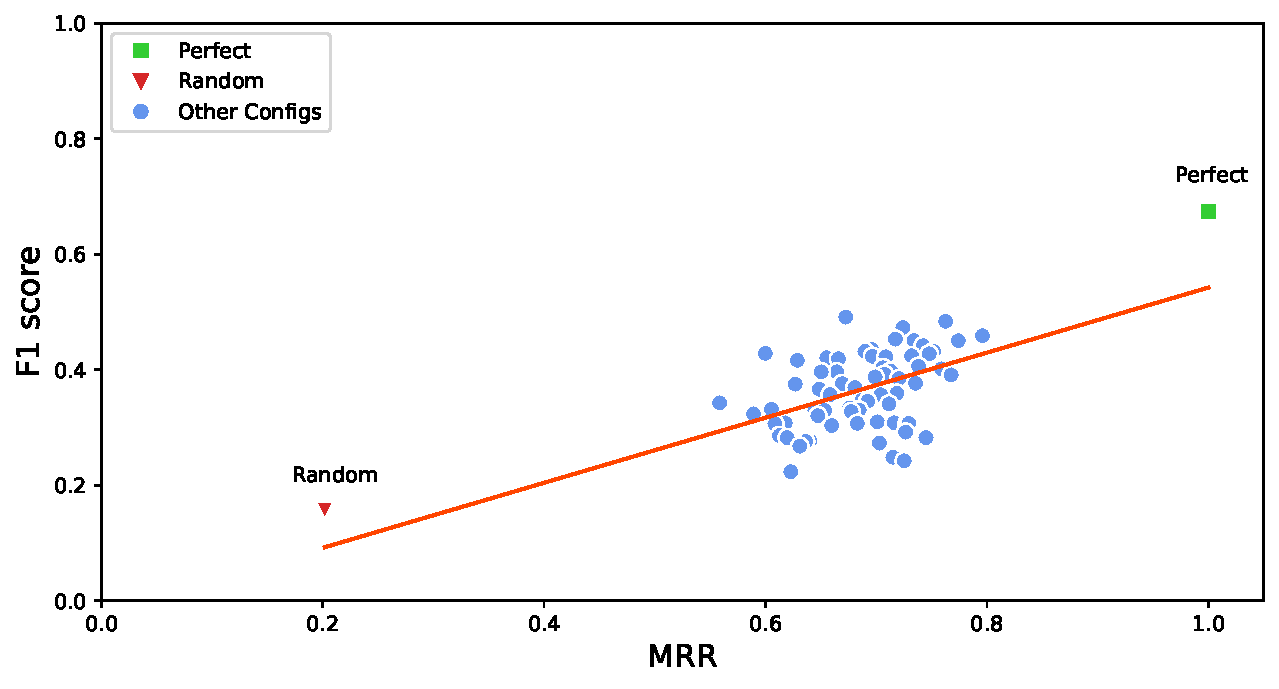
\includegraphics[width=1\linewidth]{images/MRR_craftdroid_all_oracle_included.pdf}
		\caption{\craftdroid as selector}
		\label{fig:MRR_craftdroid_all_oracle_full}
	\end{subfigure}%
	\begin{subfigure}{.5\textwidth}
		\centering
		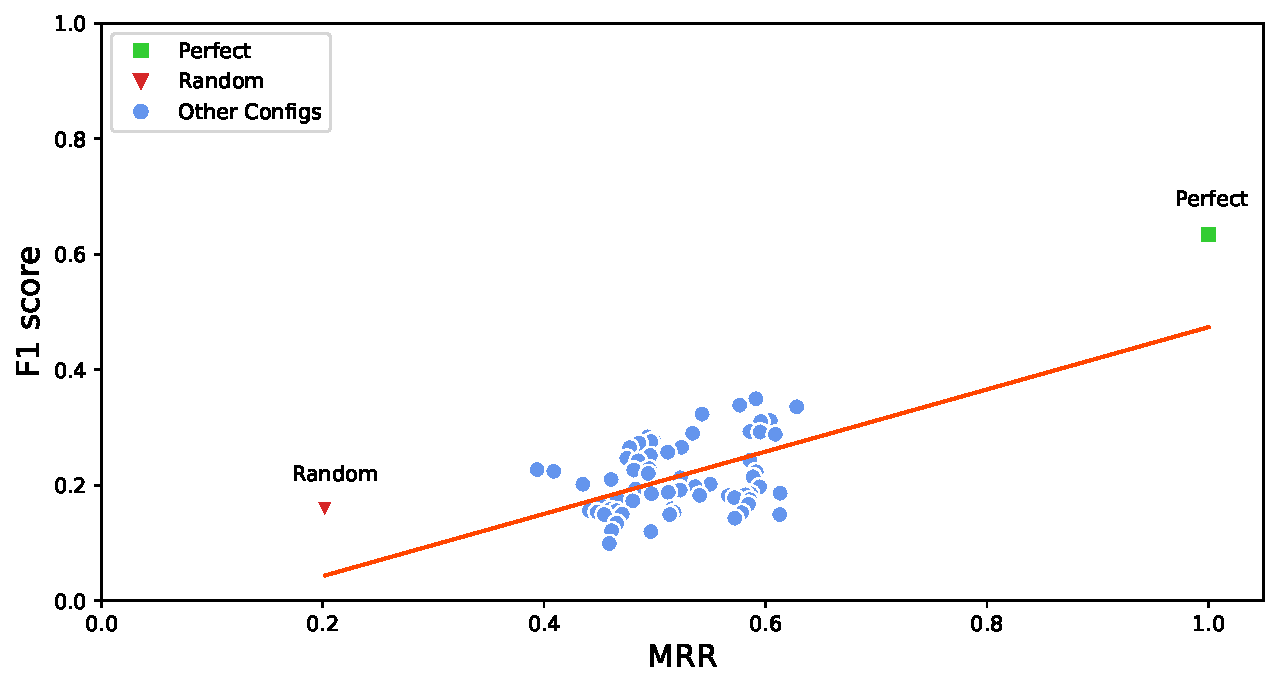
\includegraphics[width=1\linewidth]{images/MRR_atm_atm_oracle_included_passfree.pdf}
		\caption{ ATM as selector}
		\label{fig:MRR_atm_atm_oracle_passfree_full.pdf}
	\end{subfigure}
	\caption{Correlation between semantic matching (\mrr) and \testreuse (\fscore)}
	\label{fig:MRR-F1-scatter}
\end{figure}

\noindent
\textbf{Professional Competence:}

\noindent
The applicant gained research competence the subject of this project, \testreuse, in his PhD studies.
The applicant has obtained the relevant IT skills and knowledge in relevant areas during his undergraduate and graduate studies in software engineering.














